\documentclass[brazil,times,12pt]{abnt}
\usepackage[T1]{fontenc}
\usepackage[utf8]{inputenc}
\usepackage{url}
\usepackage{graphicx}
\usepackage{float}
\usepackage[pdfborder={0 0 0}]{hyperref}
\makeatletter
\usepackage{babel}
\makeatother
\begin{document}

\autor{Pedro Paulo Vezzá Campos}

\titulo{Simulação de rede de computadores utilizando OPNET IT Guru Academic
Edition}

\comentario{Trabalho apresentado para avaliação na disciplina INE5414, do
curso de Bacharelado em Ciências da Computação, turma 04208, da Universidade   
Federal de Santa Catarina, ministrada pelo professor Carlos Becker Westphall}

\instituicao{Departamento de Informática e Estatística \par Centro
Tecnológico \par Universidade Federal de Santa Catarina}

\local{Santa Catarina - SC, Brasil}

\data{\today}

\capa

\folhaderosto

% \tableofcontents
%\chapter{}
\section*{Objetivos}
Para este terceiro trabalho prático foi proposto que fosse simulada a rede
previamente analisada no segundo trabalho prático (\cite{campos:pratica-gerencia-redes}) utizando uma
ferramenta de gerência SNMP. Para isso, os alunos deveriam utilizar uma
ferramenta de simulação de redes, e ao final apresentassem gráficos relacionados
ao desempenho da rede escolhida.

Neste trabalho será apresentada primeiramente uma introdução à simulação de
redes, seguida da apresentação das ferramentas utilizadas no experimento.
Posteriormente, serão apresentadas a topologia da rede modelada, as
configurações adotadas na ferramenta, os gráficos resultantes da simulação,
algumas restrições à análise das informações e por fim uma conclusão.

\section*{Introdução à Simulação de Redes}
A simulação de redes pode ser vista como uma tentativa de modelar redes de
computadores reais. A partir do momento que essa simulação é fidedigna o
suficiente diante da realidade, ela torna-se uma poderosa ferramenta no arsenal
de um gerente de redes capacitado. Através dela, pode-se modelar
com custos nulos ou muito baixos diferentes modelos de redes, coletando
informações relevantes, que permitem ao gerente determinar a melhor arquitetura
de redes possível sem incorrer nos gastos elevados de uma implantação real.
\cite{wiki:network-simulation}

Uma restrição da simulação de redes é a necessidade da aproximação dos fluxos de
dados a variáveis estatísticas. As ferramentas de redes oferecem diferentes
modelos de distribuição de dados, desde os mais simples, como a distribuição
uniforme até modelos mais elaborados como normal, hipergeométrica, poisson,
dentre outras. Uma consequência dessa abordagem, aliado à necessidade da
discretização dos eventos simulados, é que as simulações de rede não são
perfeitas. Porém, como dito anteriormente, podem ser boas aproximações,
permitindo uma relação custo-benefício entre nível de fidelidade e custo de
simulação vantajoso. \cite{hughes:network-simulation-introduction}

\section*{Experimento Prático}
\subsection*{Recursos Utilizados}
\begin{description}
  \item[Windows 7] Sistema operacional adotado, versão Professional 64 bits.
  \item[OPNET IT Guru Academic Edition] Simulador de redes escolhido.
\end{description}

\subsection*{Detalhamento do experimento}
Diante da acentuada curva de aprendizado necessária para dominar o
Network Simulator (ns-2), foi adotado o OPNET IT Guru Academic Edition como
ferramenta de simulação de redes. Como vantagens ao seu uso, incluem-se a
facilidade de uso de sua interface com usuário, relativa disponibilidade de
documentação na Internet. Já como desvantagens há o fato de ser uma ferramenta
defasada em sua versão acadêmica, não possuindo disponibilidade dos protocolos
802.11g ou 802.11n, por exemplo.

Após a instalação do OPNET, procedeu-se ao estudo de seu uso. Dentre as
documentações mais úteis incluem-se \cite{opnet:small-network} e
\cite{siddique:wlan-opnet-tutorial} com a ressalva que mesmo seguindo todas as
instruções fornecidas por \cite{siddique:wlan-opnet-tutorial} a ferramenta
aparentemente divergia, informando que necessitaria de mais de 2000 horas para
simular uma hora de tráfego de rede.


\subsection*{Topologia da Rede}
A topologia da rede é composta por 6 estações de trabalho ligadas a um
\emph{access-point}, esse ligado à Internet. Devido à indisponibilidade do
protocolo 802.11g, adotado na rede real, procedeu-se com a simulação assumindo
uma rede 802.11.b, a 11 Mbps. O desenho resultante da topologia encontra-se
abaixo:

%\usepackage{graphics} is needed for \includegraphics
\begin{figure}[htp]
\begin{center}
  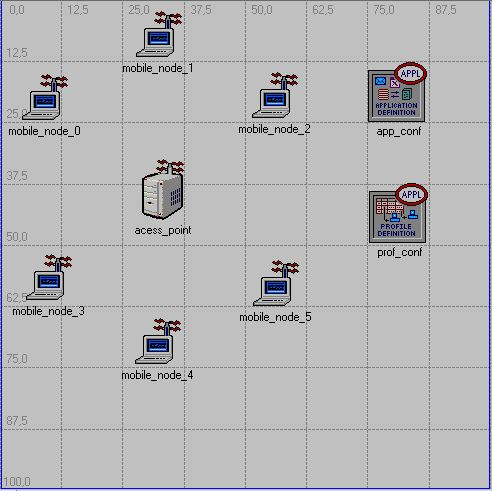
\includegraphics[width=90mm]{SimulacaoRede/Topologia.jpg}
  \caption[topologia-rede]{Topologia da rede simulada}
  \label{topologia-rede}
\end{center}
\end{figure}

\subsection*{Configurações Adotadas}
Para a simulação do tráfego, foi necessário aproximar o tráfego da rede real,
bastante heterogêneo, composto de transmissões HTTP, streamings, E-mail,
BitTorrent, FTP, VoIP, clientes de bate-papo, dentre outros, para alguns poucos
na ferramenta de simulação. Especificamente foram adotados as seguintes fontes de tráfego:

\begin{itemize}
  \item Tráfego HTTP intenso (Páginas da WWW, streamings, VoIP, etc.)
  \item Tráfego de troca de arquivos (FTP) intenso (BitTorrent, FTP, etc.)
  \item Tráfego de e-mail leve (Outros protocolos de menor relevância)
\end{itemize}

%\usepackage{graphics} is needed for \includegraphics
\begin{figure}[htp]
\begin{center}
  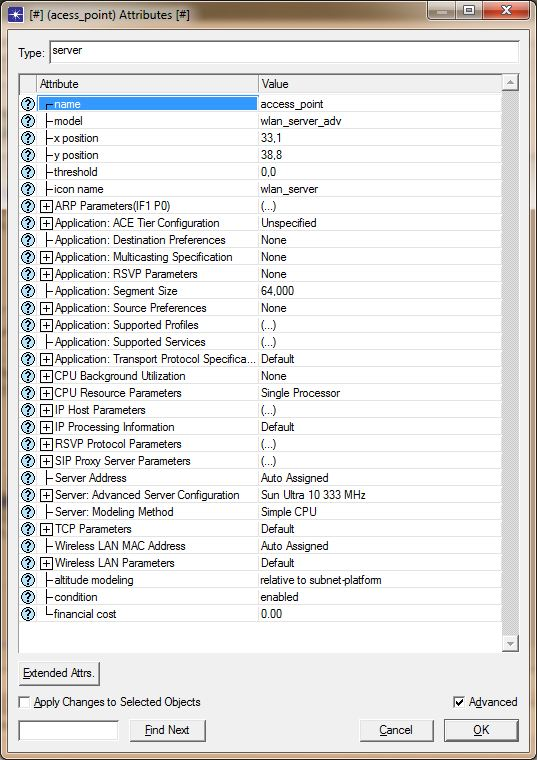
\includegraphics[width=90mm]{SimulacaoRede/AccessPointConf.jpg}
  \caption[access-point-conf]{Configuração do \emph{Access-Point}}
  \label{access-point-conf}
\end{center}
\end{figure}

%\usepackage{graphics} is needed for \includegraphics
\begin{figure}[htp]
\begin{center}
  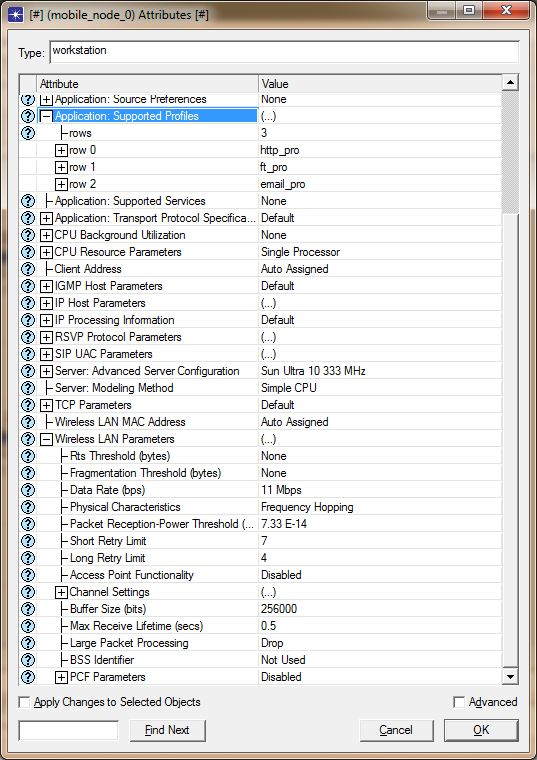
\includegraphics[width=90mm]{SimulacaoRede/WorkstationConf.jpg}
  \caption[workstation-conf]{Configuração da Estação de trabalho}
  \label{workstation-conf}
\end{center}
\end{figure}

%\usepackage{graphics} is needed for \includegraphics
\begin{figure}[htp]
\begin{center}
  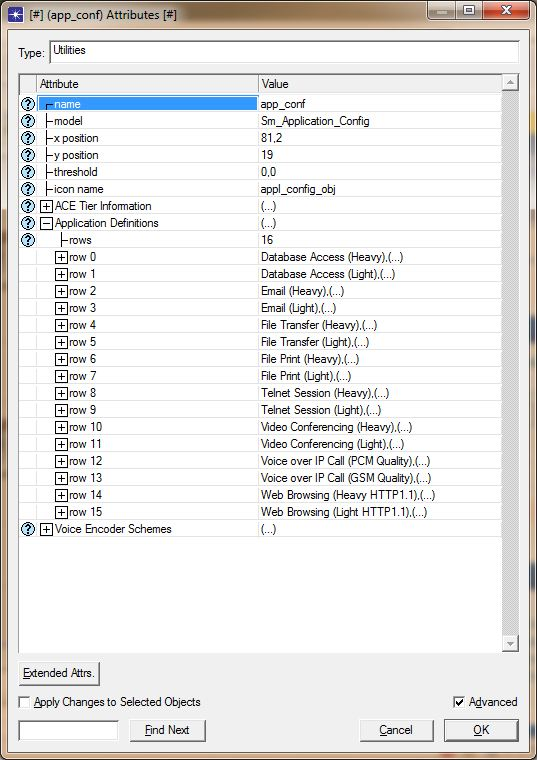
\includegraphics[width=90mm]{SimulacaoRede/AppConf.jpg}
  \caption[app-def-conf]{Configuração do \emph{Application Definition}}
  \label{app-def-conf}
\end{center}
\end{figure}

%\usepackage{graphics} is needed for \includegraphics
\begin{figure}[htp]
\begin{center}
  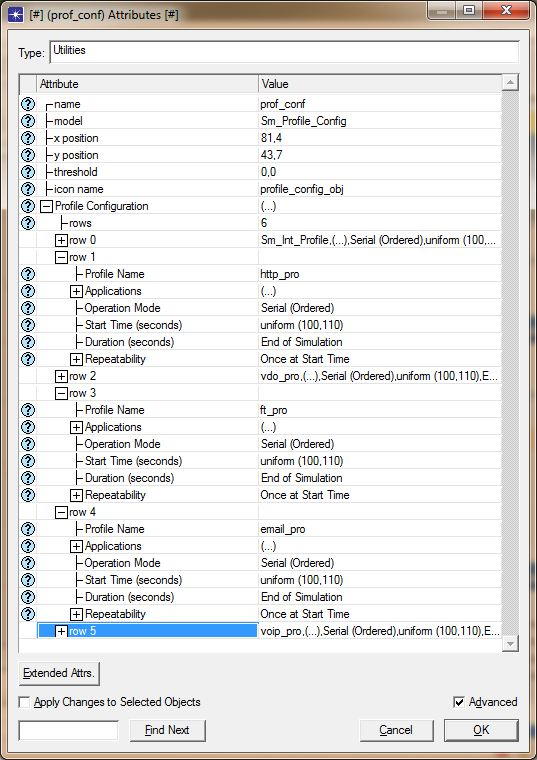
\includegraphics[width=90mm]{SimulacaoRede/ProfConf.jpg}
  \caption[prof-def-conf]{Configuração do \emph{Profile Definition}}
  \label{prof-def-conf}
\end{center}
\end{figure}

\subsection*{Gráficos de Simulação Resultantes}
Os gráficos de simulação abaixo são o resultado da simulação de 24h de uso da
rede, tal como descrito no segundo trabalho prático.

\subsubsection*{Gráficos de desempenho global}

%\usepackage{graphics} is needed for \includegraphics
\begin{figure}[htp]
\begin{center}
  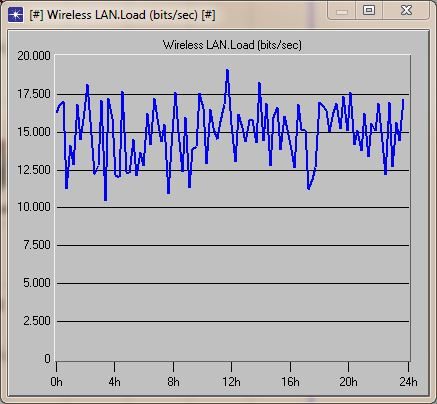
\includegraphics[width=80mm]{SimulacaoRede/CargaWifi.jpg}
  \caption[carga-wifi]{Carga na rede WiFi}
  \label{carga-wifi}
\end{center}
\end{figure}

%\usepackage{graphics} is needed for \includegraphics
\begin{figure}[htp]
\begin{center}
  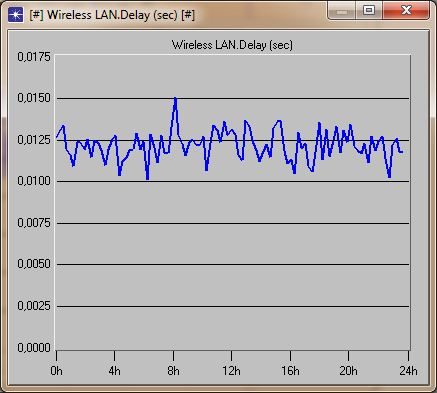
\includegraphics[width=80mm]{SimulacaoRede/DelayWifi.jpg}
  \caption[delay-wifi]{Delay na rede WiFi}
  \label{delay-wifi}
\end{center}
\end{figure}

%\usepackage{graphics} is needed for \includegraphics
\begin{figure}[htp]
\begin{center}
  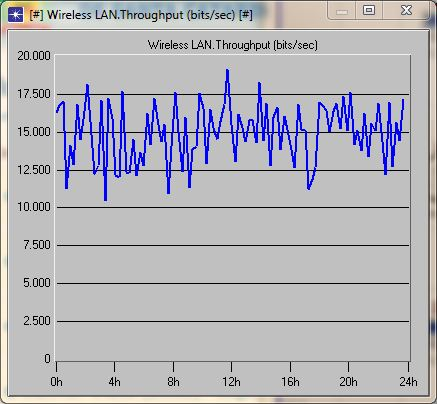
\includegraphics[width=80mm]{SimulacaoRede/ThroughputWifi.jpg}
  \caption[throughput-wifi]{Throughput na rede WiFi}
  \label{throughput-wifi}
\end{center}
\end{figure}

%\usepackage{graphics} is needed for \includegraphics
\begin{figure}[htp]
\begin{center}
  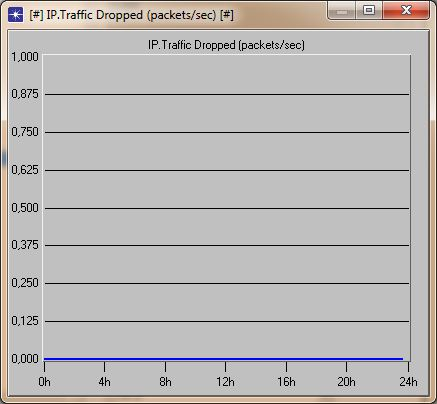
\includegraphics[width=80mm]{SimulacaoRede/TrafegoDropped.jpg}
  \caption[dropped-wifi]{\emph{Dropped Packets} na rede WiFi}
  \label{dropped-wifi}
\end{center}
\end{figure}

%\usepackage{graphics} is needed for \includegraphics
\begin{figure}[htp]
\begin{center}
  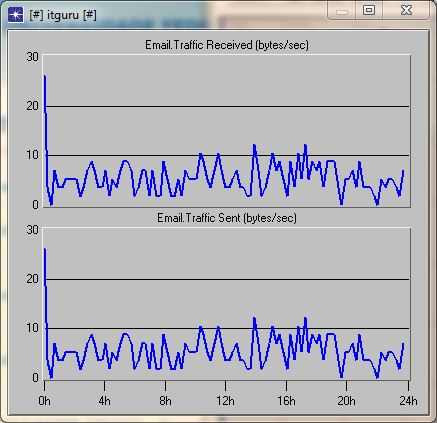
\includegraphics[width=80mm]{SimulacaoRede/TrafegoEmail.jpg}
  \caption[trafego-email]{Tráfego de entrada e saída de emails}
  \label{trafego-email}
\end{center}
\end{figure}

%\usepackage{graphics} is needed for \includegraphics
\begin{figure}[htp]
\begin{center}
  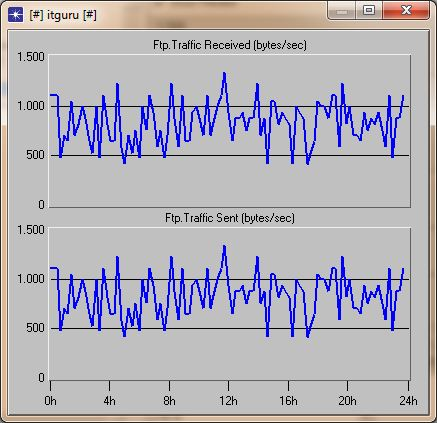
\includegraphics[width=80mm]{SimulacaoRede/TrafegoFTP.jpg}
  \caption[trafego-ftp]{Tráfego de entrada e saída FTP}
  \label{trafego-ftp}
\end{center}
\end{figure}

%\usepackage{graphics} is needed for \includegraphics
\begin{figure}[htp]
\begin{center}
  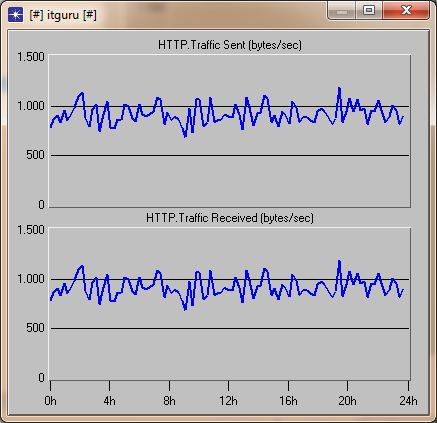
\includegraphics[width=80mm]{SimulacaoRede/TrafegoHTTP.jpg}
  \caption[trafego-http]{Tráfego de entrada e saída HTTP}
  \label{trafego-http}
\end{center}
\end{figure}

\subsubsection*{Gráficos de nodos individuais}

%\usepackage{graphics} is needed for \includegraphics
\begin{figure}[H]
\begin{center}
  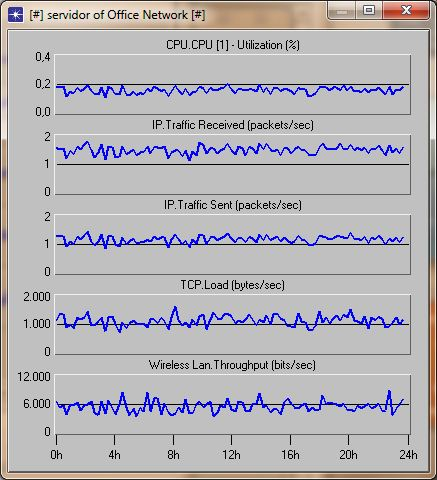
\includegraphics[width=80mm]{SimulacaoRede/AccessPoint.jpg}
  \caption[trafego-access-point]{Informações de tráfego no access-point}
  \label{trafego-access-point}
\end{center}
\end{figure}

%\usepackage{graphics} is needed for \includegraphics
\begin{figure}[H]
\begin{center}
  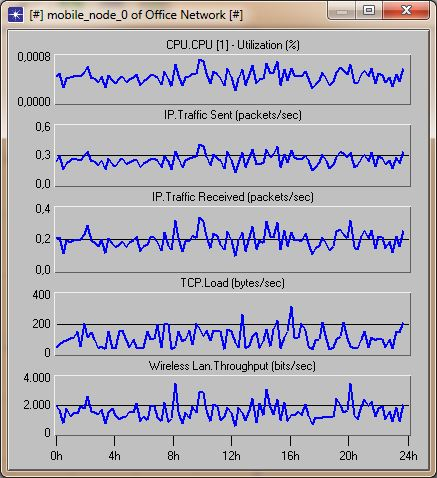
\includegraphics[width=80mm]{SimulacaoRede/Maquina0.jpg}
  \caption[trafego-maquina0]{Informações de tráfego na máquina 0}
  \label{trafego-maquina0}
\end{center}
\end{figure}

%\usepackage{graphics} is needed for \includegraphics
\begin{figure}[H]
\begin{center}
  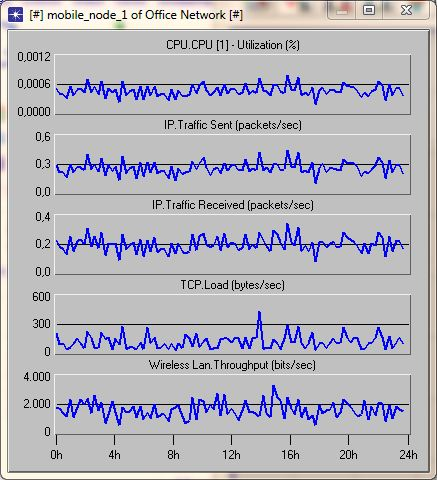
\includegraphics[width=80mm]{SimulacaoRede/Maquina1.jpg}
  \caption[trafego-maquina1]{Informações de tráfego na máquina 1}
  \label{trafego-maquina1}
\end{center}
\end{figure}

%\usepackage{graphics} is needed for \includegraphics
\begin{figure}[H]
\begin{center}
  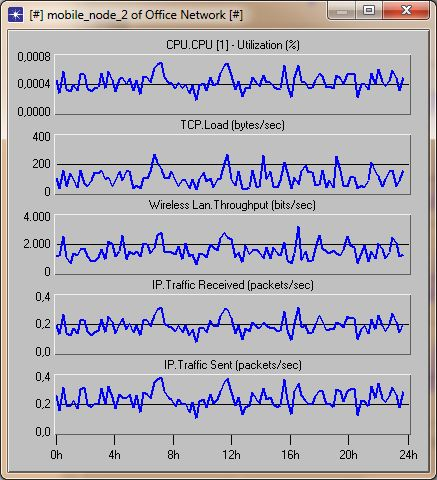
\includegraphics[width=80mm]{SimulacaoRede/Maquina2.jpg}
  \caption[trafego-maquina2]{Informações de tráfego na máquina 2}
  \label{trafego-maquina2}
\end{center}
\end{figure}

%\usepackage{graphics} is needed for \includegraphics
\begin{figure}[H]
\begin{center}
  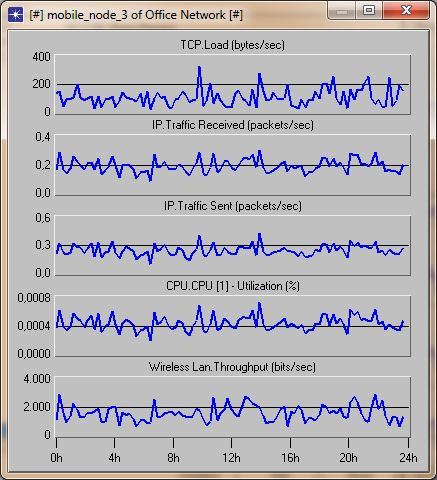
\includegraphics[width=80mm]{SimulacaoRede/Maquina3.jpg}
  \caption[trafego-maquina3]{Informações de tráfego na máquina 3}
  \label{trafego-maquina3}
\end{center}
\end{figure}

%\usepackage{graphics} is needed for \includegraphics
\begin{figure}[H]
\begin{center}
  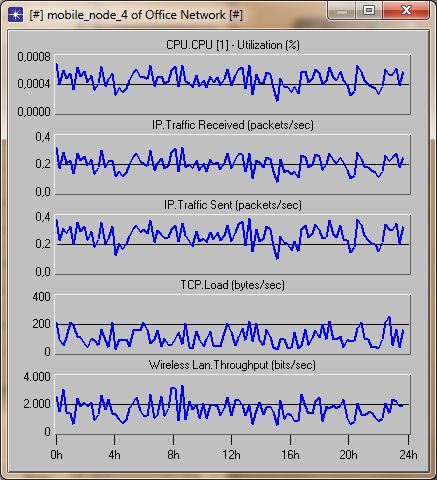
\includegraphics[width=80mm]{SimulacaoRede/Maquina4.jpg}
  \caption[trafego-maquina4]{Informações de tráfego na máquina 4}
  \label{trafego-maquina4}
\end{center}
\end{figure}

%\usepackage{graphics} is needed for \includegraphics
\begin{figure}[H]
\begin{center}
  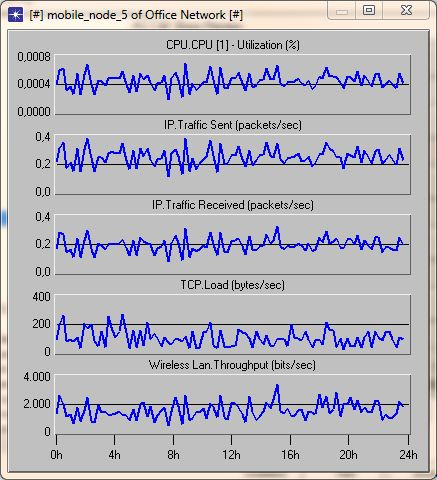
\includegraphics[width=80mm]{SimulacaoRede/Maquina5.jpg}
  \caption[trafego-maquina5]{Informações de tráfego na máquina 5}
  \label{trafego-maquina5}
\end{center}
\end{figure}

\subsection*{Limitações da Simulação}
Como dito anteriormente, a simulação possui algumas limitações, ou de ordem
prática ou de limitação da ferramenta. Algumas delas são: Necessidade de uso de
simulação 802.11b, ao invés de 802.11g, aproximação de fluxos de dados
heterogêneos por poucos fluxos simulados e aproximação do uso da rede durante as
24 horas simuladas. Todas essas alterações podem afetar as informações coletadas
durante o trabalho.

\section*{Conclusão}
O terceiro trabalho prático proposto pelo professor Westphall foi de grande
valia para o aluno adquirir habilidade com uma ferramenta de simulação de rede,
um conhecimento importante para um acadêmico de Redes de Computadores I e
essencial para um aspirante a gerente de redes.

Através desse trabalho o aluno pode experimentar diversos problemas inerentes à
tarefa de simulação de redes, permitindo aproveitar diversos conceitos
adquiridos durante o semestre, tais como as camadas do modelo OSI, gerência de
redes, além de estimular o estudo de quaisquer temas importantes ao
trabalho de maneira dirigida.

\bibliographystyle{abnt-num}
\bibliography{bibliografia}
\end{document}